\documentclass{beamer}
\usepackage[utf8]{inputenc}

\usetheme{Madrid}
\usecolortheme{default}
\usepackage{amsmath,amssymb,amsfonts,amsthm}
\usepackage{mathtools}
\usepackage{txfonts}
\usepackage{tkz-euclide}
\usepackage{listings}
\usepackage{adjustbox}
\usepackage{tfrupee}
\usepackage{array}
\usepackage{gensymb}
\usepackage{tabularx}
\usepackage{gvv}
\usepackage{lmodern}
\usepackage{circuitikz}
\usepackage{tikz}
\lstset{literate={·}{{$\cdot$}}1 {λ}{{$\lambda$}}1 {→}{{$\to$}}1}
\usepackage{graphicx}

\setbeamertemplate{page number in head/foot}[totalframenumber]

\usepackage{tcolorbox}
\tcbuselibrary{minted,breakable,xparse,skins}

\definecolor{bg}{gray}{0.95}
\DeclareTCBListing{mintedbox}{O{}m!O{}}{%
  breakable=true,
  listing engine=minted,
  listing only,
  minted language=#2,
  minted style=default,
  minted options={%
    linenos,
    gobble=0,
    breaklines=true,
    breakafter=,,
    fontsize=\small,
    numbersep=8pt,
    #1},
  boxsep=0pt,
  left skip=0pt,
  right skip=0pt,
  left=25pt,
  right=0pt,
  top=3pt,
  bottom=3pt,
  arc=5pt,
  leftrule=0pt,
  rightrule=0pt,
  bottomrule=2pt,
  toprule=2pt,
  colback=bg,
  colframe=orange!70,
  enhanced,
  overlay={%
    \begin{tcbclipinterior}
    \fill[orange!20!white] (frame.south west) rectangle ([xshift=20pt]frame.north west);
    \end{tcbclipinterior}},
  #3,
}
\lstset{
    language=C,
    basicstyle=\ttfamily\small,
    keywordstyle=\color{blue},
    stringstyle=\color{orange},
    commentstyle=\color{green!60!black},
    numbers=left,
    numberstyle=\tiny\color{gray},
    breaklines=true,
    showstringspaces=false,
}

\title{10.3.12}
\date{September 29, 2025}
\author{Bhargav - EE25BTECH11013}

\begin{document}

\frame{\titlepage}

\begin{frame}{Question}
\textbf{Question}: \\
If the line $y = \sqrt{3}x + K$ touches the parabola $x^2 = 16y$, then find the value of K.\\ \\
\end{frame}
\begin{frame}{Solution}
The equation of the conic $\brak{parabola}$ can be written as
\begin{align}
\vec{x^T}\vec{V}\vec{x} + 2\vec{u^T}\vec{x} + f = 0
\end{align}
\begin{align}
\vec{V} = \myvec{1 & 0 \\ 0 & 0}, \vec{u} = \myvec{0 \\ -8}, f=0, \vec{m^T} = \myvec{1 \\ \sqrt{3}}
\end{align}
\begin{align}
\vec{x} = \vec{h} + k_i\vec{m}    
\end{align}

The value of $k_i$ can be found out by solving the line and conic equation

\begin{align}
(\vec{h} + k_i \vec{m})^{\top} \vec{V} (\vec{h} + k_i \vec{m}) + 2\vec{u}^{\top} (\vec{h} + k_i \vec{m}) + f &= 0 \\
\implies k_i^{2} \vec{m}^{\top}\vec{V}\vec{m} + 2k_i \vec{m}^{\top} (\vec{V}\vec{h} + \vec{u}) + \vec{h}^{\top}\vec{V}\vec{h} + 2\vec{u}^{\top}\vec{h} + f &= 0 \\
\text{or, } k_i^{2} \vec{m}^{\top}\vec{V}\vec{m} + 2k_i \vec{m}^{\top} (\vec{V}\vec{h} + \vec{u}) + g(\vec{h}) &= 0
\end{align}



\end{frame}

\begin{frame}{Solution}

Solving the above quadratic gives the equation
\begin{align}
k_i = \frac{1}{\vec{m}^{\top}\vec{V}\vec{m}}
\brak{
    -\vec{m}^{\top} (\vec{V}\vec{h} + \vec{u})
    \;\pm\;
    \sqrt{ \sbrak{\vec{m}^{\top}(\vec{V}\vec{h} + \vec{u})}^2
    - g(\vec{h}) \, (\vec{m}^{\top}\vec{V}\vec{m}) }
    }
\end{align}
Since the tangent passes through one point of the conic, and $g\brak{\vec{q}}=0$
\begin{align}
\vec{m^T}\brak{\vec{\vec{V}\vec{q} + \vec{u}}} = 0
\end{align}
\begin{align}
\vec{m^T}\vec{V}\vec{q} = -\vec{m^T}\vec{u}
\end{align}
\begin{align}
\vec{q} = -\frac{\brak{\vec{m^T}\vec{V}}^T\vec{m^T}\vec{u}}{\norm{\vec{m^T}\vec{V}}^2}
\end{align}

On solving, we get
\begin{align}
\vec{q} = \myvec{8\sqrt{3} \\ t}, t \in \mathbf{R}
\end{align}
\end{frame}

\begin{frame}{Solution}
Since $\vec{q}$ lies on the conic, 
\begin{align}
g\brak{\vec{\vec{q}}} = 0
\end{align}
\begin{align}
\implies \vec{q^T}\vec{V}\vec{q} + 2\vec{u^T}\vec{q} + f = 0
\end{align}

Substituting and solving gives $t=12$

\begin{align}
\therefore \vec{q} = \myvec{8\sqrt{3} \\ 12}
\end{align}

Therefore $k = -12$    
\end{frame}

\begin{frame}{Plot}
\begin{figure}[h!]
    \centering
    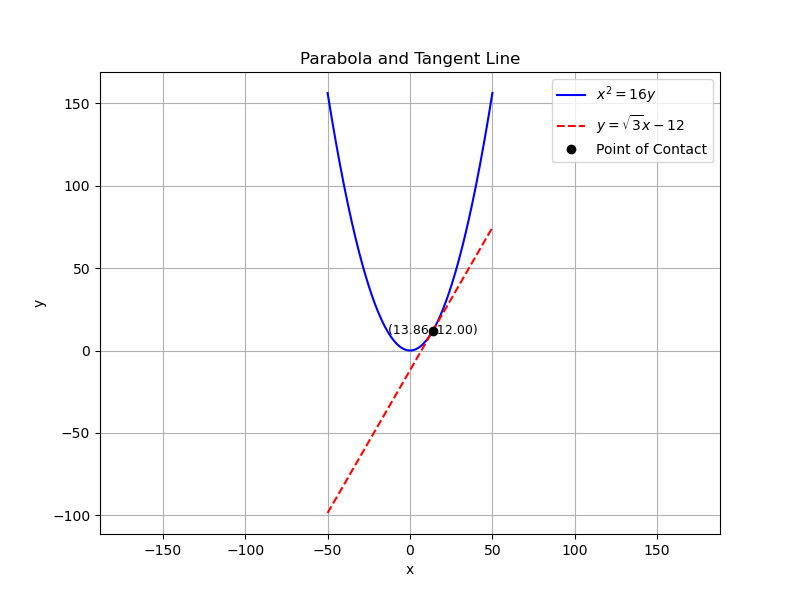
\includegraphics[height=0.5\textheight, keepaspectratio]{figs/Figure_1.png}
    \label{figure_1}
\end{figure}
\end{frame}

\begin{frame}[fragile]
    \frametitle{C Code}
    \begin{lstlisting}
#include <math.h>

double compute_x() {
    return 8 * sqrt(3);
}

double compute_y(double x) {
    return (x * x) / 16.0;
}

double compute_k(double x, double y) {
    return y - sqrt(3) * x;
}

    \end{lstlisting}
\end{frame}
\begin{frame}[fragile]
    \frametitle{Python + C Code}
    \begin{lstlisting}
import ctypes
import numpy as np
import matplotlib.pyplot as plt
lib = ctypes.CDLL('./libcode.so')
lib.compute_x.argtypes = []
lib.compute_x.restype = ctypes.c_double
lib.compute_y.argtypes = [ctypes.c_double]
lib.compute_y.restype = ctypes.c_double
lib.compute_k.argtypes = [ctypes.c_double, ctypes.c_double]
lib.compute_k.restype = ctypes.c_double
x = lib.compute_x()
y = lib.compute_y(x)
K = lib.compute_k(x, y)
q = np.array([x, y])
x_vals = np.linspace(-50, 50, 400)
y_parabola = x_vals**2 / 16
    \end{lstlisting}
\end{frame}
\begin{frame}[fragile]
    \frametitle{Python + C Code}
    \begin{lstlisting}
y_line = np.sqrt(3) * x_vals + K
plt.figure(figsize=(8, 6))
plt.plot(x_vals, y_parabola, label=r'$x^2 = 16y$', color='blue')
plt.plot(x_vals, y_line, label=rf'$y = \sqrt{{3}}x {K:.0f}$', color='red', linestyle='--')
plt.plot(q[0], q[1], 'ko', label='Point of Contact')
plt.text(q[0], q[1], f'({q[0]:.2f}, {q[1]:.2f})', fontsize=9, ha='center', va='center')
plt.title("Parabola and Tangent Line")
plt.xlabel("x")
plt.ylabel("y")
plt.legend()
plt.grid(True)
plt.axis('equal')
plt.savefig("/mnt/c/Users/bharg/Documents/backupmatrix/ee25btech11013/matgeo/10.3.12/figs/Figure_1.png")
plt.show()



    \end{lstlisting}
\end{frame}
\begin{frame}[fragile]
    \frametitle{Python Code}
    \begin{lstlisting}
import numpy as np
import matplotlib.pyplot as plt

V = np.array([[1, 0], [0, 0]])
u = np.array([[0], [-8]])
f = 0
m = np.array([[1], [np.sqrt(3)]])
x = 8 * np.sqrt(3)
y = x**2 / 16
q = np.array([x, y])
K = y - np.sqrt(3) * x
x_vals = np.linspace(-50, 50, 400)
y_parabola = x_vals**2/16
y_line = np.sqrt(3)*x_vals + K
plt.figure(figsize=(8, 6))
plt.plot(x_vals, y_parabola, label=r'$x^2 = 16y$', color='blue')
plt.plot(x_vals, y_line, label=rf'$y = \sqrt{{3}}x {K:.0f}$', color='red', linestyle='--')


    \end{lstlisting}
\end{frame}

\begin{frame}[fragile]
    \frametitle{Python Code}
    \begin{lstlisting}
plt.plot(q[0], q[1], 'ko', label='Point of Contact')
plt.text(q[0], q[1], f'({q[0]:.2f}, {q[1]:.2f})')
plt.title("Parabola and Tangent Line")
plt.xlabel("x")
plt.ylabel("y")
plt.legend()
plt.grid(True)
plt.axis('equal')
plt.savefig("/mnt/c/Users/bharg/Documents/backupmatrix/ee25btech11013/matgeo/10.3.12/figs/Figure_1.png")
plt.show()


    \end{lstlisting}
\end{frame}
\end{document}

